% !TeX encoding = UTF-8
% !TeX spellcheck = en_US
% !TeX root = ../../Thesis.tex

\chapter{Vacuum test chamber}
\label{ch:Vacuum chamber}

In order to be able to fit the CRT screen, CF160 flanges were chosen for the test chamber. At one point during testing, major changes were made which will be explained in \cref{sec:Second iteration}.

\correction{explain more in detail what is the purpose of the chamber, the two iterations are not really important built this chapter rather about the function and operation of the chamber over time due to outgasing the pressure improved)}
\section{First iteration}
\label{sec:vacuum chamber first iteration}

A 3D render of the chamber is shown in  (\cref{fig:3D rendering of test chamber}). Without a CRT installed, it was possible to reach a pressure of \SI{6.8e-7}{\milli\bar}. With a CRT installed inside, the lowest achieved pressure was \SI{2.0e-6}{\milli\bar}. It was not possible to reach a lower pressure due to outgassing.

 
\subsection{Chamber Setup}
\label{subsec:Chamber Setup}
 
The center piece consists of a 6-way cross with view ports at the front and bottom. A valve was installed at the back in order to flood the chamber with nitrogen  (Alphagaz\texttrademark  N$_2$ purity $\ge\SI{99.999}{\percent}$) when installing a new CRT to reduce oxygen poisoning and avoid water vapor getting into the chamber \correction{water vapor getting into the chamber}. On the right side, a HiCube 300 Eco turbo pump was installed and on the left side a wobble stick was attached with a wire. A straight CF100 pipe of length \SI{27}{\centi\meter} was installed at the top with a 5 port cluster flange, each being of type CF40. \correction{explain in connection of the rendering; this makes it easier, if necessary you can get more renderings}

The center piece consists of a 6-way cross with view ports at the front and bottom. A valve was installed at the back in order to flood the chamber with nitrogen\todo{pure nitrogen name?} \suggestion{Alphagaz$^{TM}$ 1 $N_2$ purity $\ge\SI{99.999}{\percent}$}, when installing a new CRT to avoid oxygen poisoning \correction{water vapor getting into the chamber}. On the right side, a HiCube 80 Eco turbo pump was installed and on the left side a wobble stick was attached with a wire . A straight CF100 pipe \todo{length=27cm} was installed at the top with a 5 port cluster flange, each being of type CF40.
 
In the middle port, a Thyracont \correction{Thyracont exact model is in one note} pressure gauge was installed. On the left, a 19 pin MIL 19 C connector was installed to supply the necessary voltages to the CRT. Two flanges were equipped with four BNC feedthroughs each. One of them was used to connect the x-, and y-plates, while the other connected to the wobble stick and aluminum foil at the CRT screen. Further explanation will be given in \cref{ch:Beam Characterization}. The last port was capped off by a blank flange.

In the middle port, a VSH \correction{Thyracont exact model is in one note}  pressure gauge was installed. On the left, a 19 pin connector \todo{how many pins and model name? MIL Type C connector} \suggestion{MIL 19 C} was installed to supply the necessary voltages to the CRT. Two flanges were equipped with four BNC feedthroughs each. One of them was used to connect do the x-, and y-plates, while the other connected to the wobble stick and aluminum foil at the CRT screen. Further explanation will be given in \cref{ch:Beam Characterization}. The last port was capped off by a blank flange.
 
For the inside wires, at first stranded copper cables were used. These were later swapped for Kapton insulated BNC cables.\todo{F: but I'm talking about first iteration} The chamber was sealed by Viton rubber gaskets which were changed to copper gaskets.
For the inside wires, standard copper cables were used \correction{we also used thin Kapton insulated BNC cable}. The chamber was sealed by rubber \suggestion{Viton, maybe also describe the specification of these type of seals} gaskets.
 
\begin{figure}[ht]
	\centering
 	
	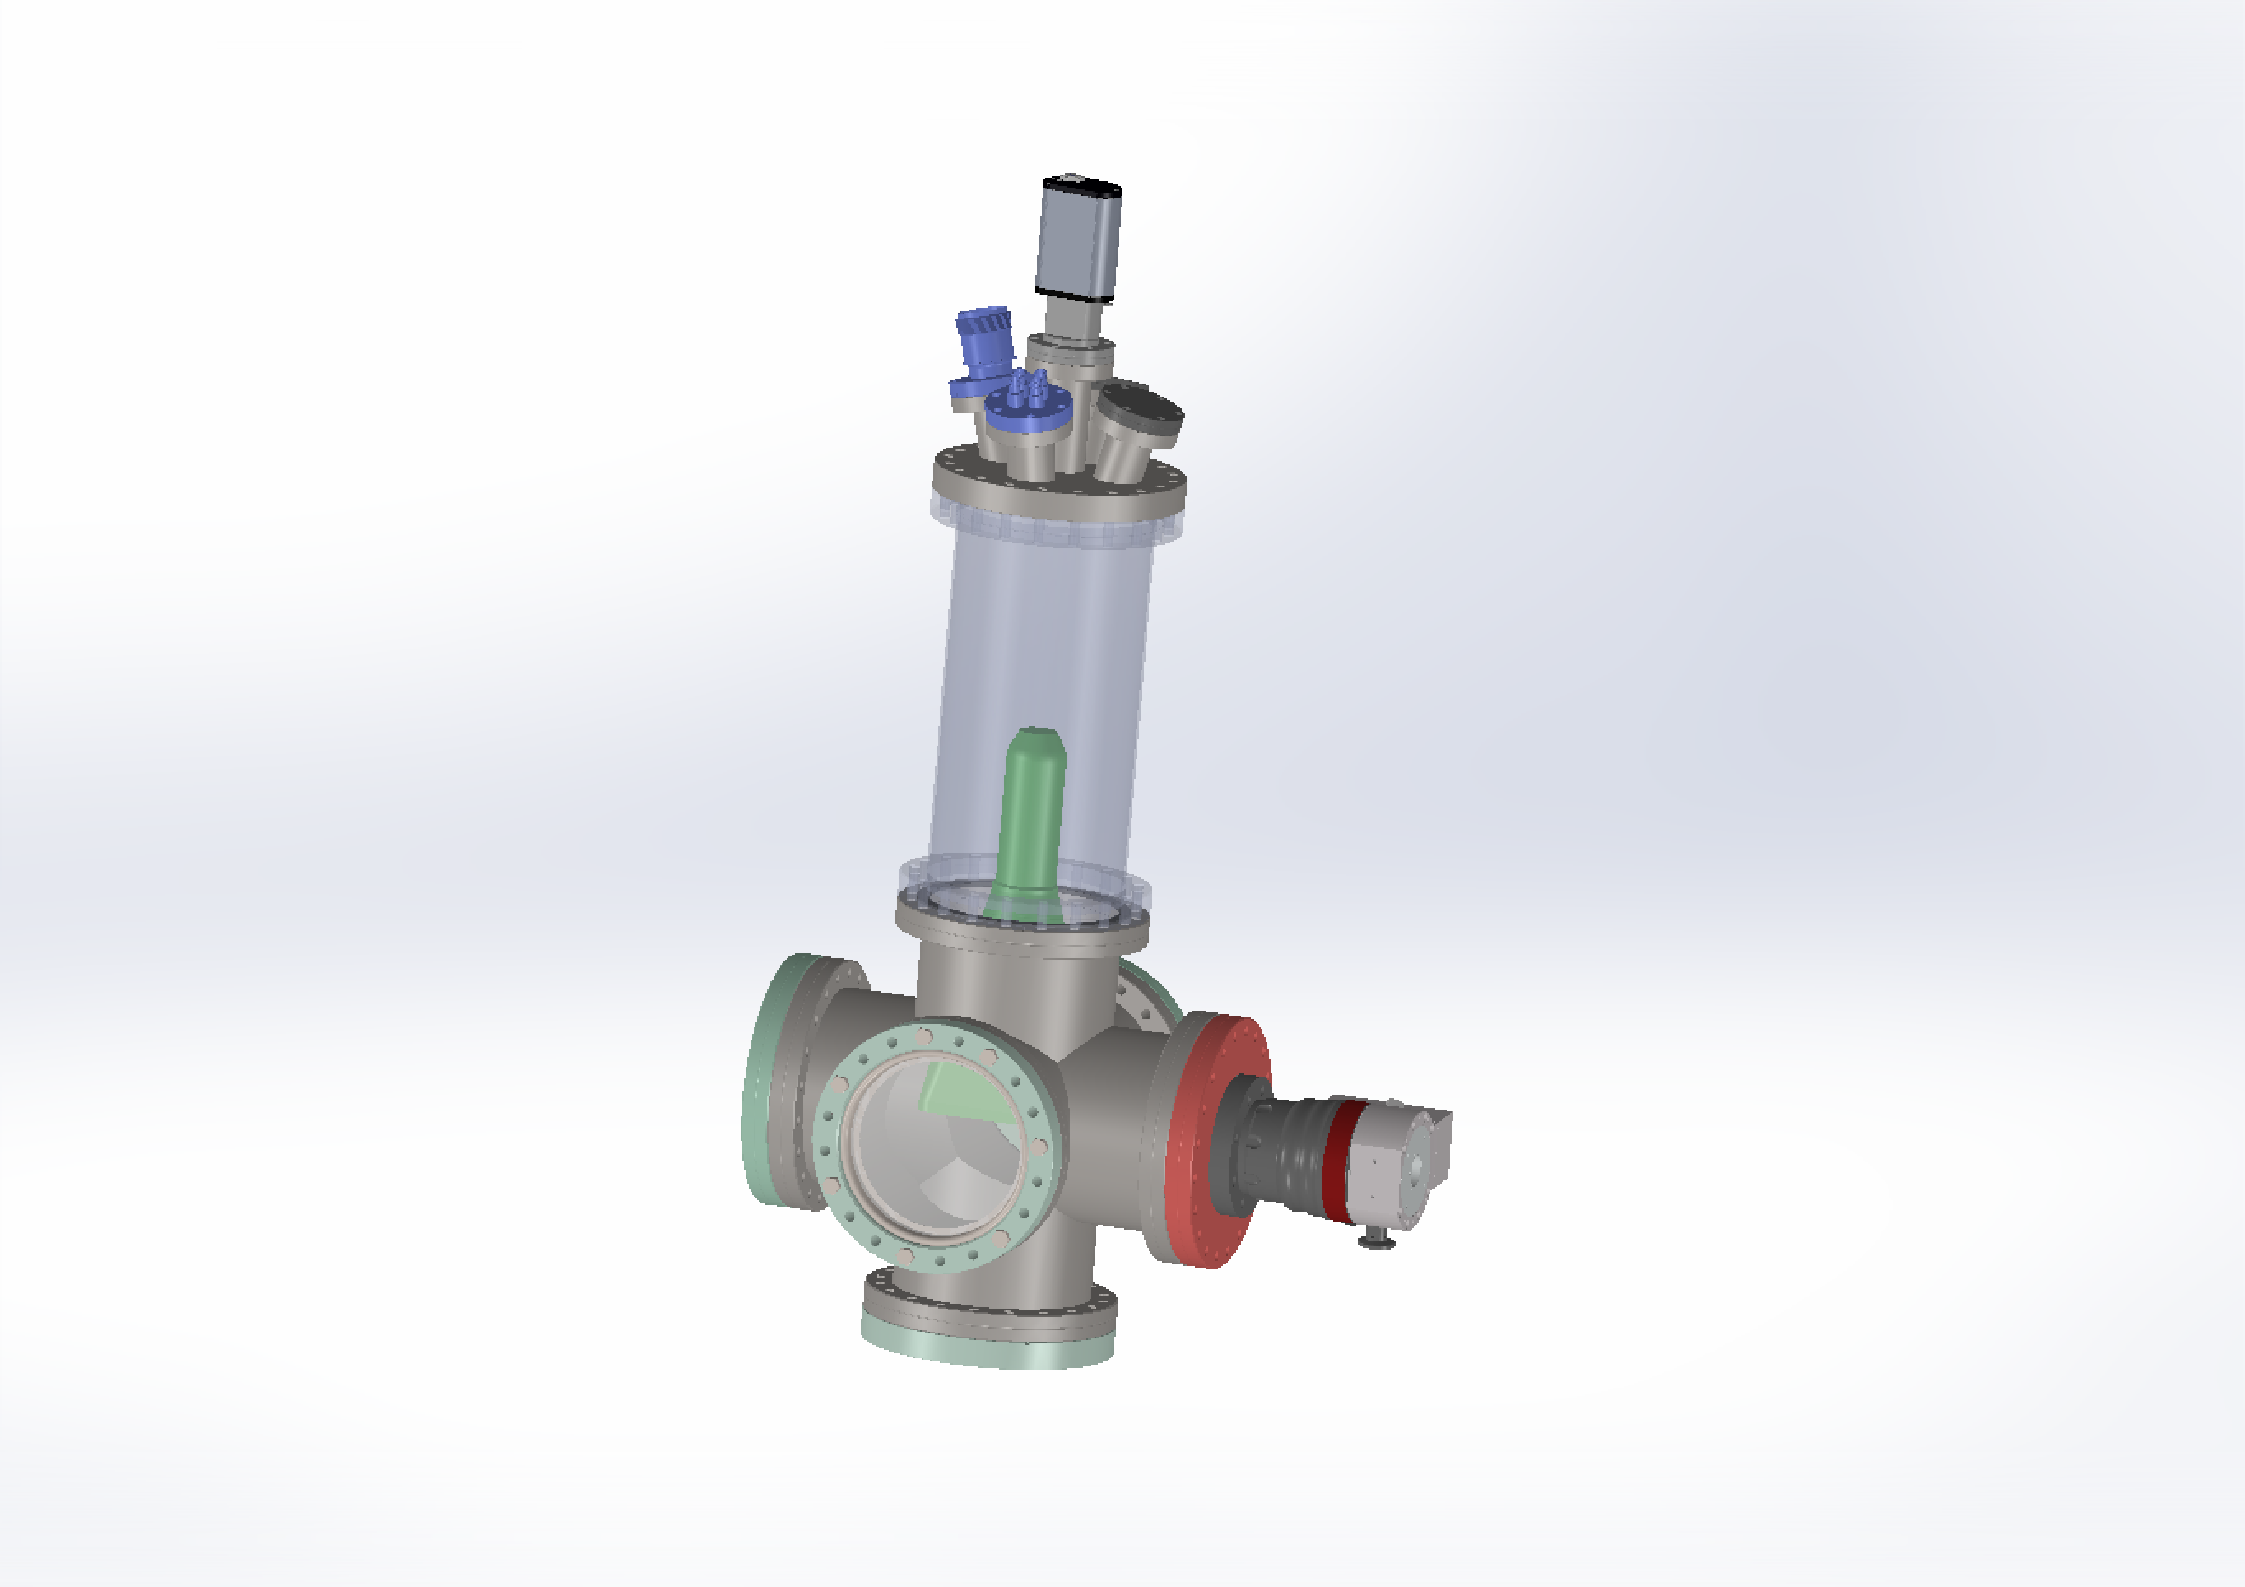
\includegraphics[width=0.9\textwidth]{./Chapters/vacuum-chamber/test_chamber} % taken from OneNote QuaK/Vacuum Setup/Test vacuum chamber
	
	\caption{3D rendering of test chamber.}
	\label{fig:3D rendering of test chamber}
\end{figure}
 
\subsection{CRT mounting mechanism}
\label{subsec:CRT mounting mechanism}

 Two M8 rods of length \todo{rod length? check Solid works} were screwed with a counter nut into the cluster flange. On each, a L shaped aluminum piece was installed between two nuts. These were then connected by a hose clamp, which was used to secure the CRT inside below the cluster flange (\cref{fig:Image of CRT mounting mechanism}).
 
 Two M8 rods of length \todo{rod length? check Solid works} were drilled \correction{screwed / with a counter nut} into the cluster flange. On each, a L shaped aluminum piece was installed between two nuts. These were then connected by a hose clamp, which was used to secure the CRT inside below the cluster flange (\cref{fig:Image of CRT mounting mechanism}).
 

\begin{figure}[h]
	\centering
	
	\missingfigure[figwidth=0.9\textwidth]{Image of CRT mounting mechanism.}
	
	\caption{Image of CRT mounting mechanism.}
	\label{fig:Image of CRT mounting mechanism}
\end{figure}


\subsection{Measurement of outgassing}
\subsection{Leak test} \correction{in general make better section titles}
\label{subsec:Measurement of outgassing}

Before inserting a CRT for the first time, measurements were made in order to find out how well low pressure could be maintained inside the chamber. First, the chamber was set to a pressure of \SI{e-5}{\milli\bar} after which the pump was turned off. The pressure was measured once a minute for a duration \SI{3}{\hour}. This is shown in \cref{fig:Time evolution of pressure inside the test chamber after turning off pump}.

Before inserting a CRT, a leak test was performed. First, the chamber was set to a pressure of \SI{e-5}{\milli\bar} after which the pump was turned off. The pressure was measured once a minute for a duration \SI{3}{\hour}. This is shown in \cref{fig:Time evolution of pressure inside the test chamber after turning off pump}. \correction{this is not so much of a leak but mainly outgasing / how was the pressure measured?}

\begin{figure}[ht]
	\centering
		
	\begin{tikzpicture}
		% !TeX encoding = UTF-8
% !TeX spellcheck = en_US
% !TeX root = ../../Thesis.tex

\begin{axis}[
	%name=zeemanShift,
	%grid=major,
	ymode = log,
	xlabel = time/\si{\minute},
	ylabel = pressure/\si{\milli\bar},
	%scaled ticks=false,
	%		every x tick scale label/.style={at={(xticklabel* cs:1.03,-0.3em)}, /pgfplots/near ticklabel align=outside, anchor=near xticklabel opposite, inner sep=0pt},
	%		xticklabel style={/pgf/number format/sci}, sci generic={mantissa sep=\cdot,exponent={10^{#1}}}},
	%yticklabel style={/pgf/number format/sci},
	xmin = 0,
	ymin = 1e-5,
	%extra tick style={grid=none}, 
	%width=0.7\textwidth,
	%legend style={at={(1.02, 0.5)}, anchor = west},
	%every axis plot/.append style={thick}
	]
	\addplot[mark=none, black] table [x=t, y=p, col sep=comma]{./Chapters/vacuum-chamber/leak_rate.csv};
\end{axis}
	\end{tikzpicture}
	
	\caption{Time evolution of pressure inside the test chamber after turning off pump.}
	\label{fig:Time evolution of pressure inside the test chamber after turning off pump}
\end{figure}


\section{Second iteration}
\label{sec:Second iteration}

At one point during experimentation, major changes were made to the chamber. Thanks to these, it was possible to reach a pressure of \SI{1.2e-7}{\milli\bar}.

\subsection{Changes}
\label{subsec:Changes}

First, every rubber gasket was exchanged to a copper one for a better seal, except at the cluster flange, since that spot will be opened and closed the most often. Each copper stranded cable inside was switched to a coaxial one and the mantle was connected to the chamber wall, which was set to ground. A Faraday cup was installed below the wobble stick, to accurately measure the beam current (further details in \cref{sec:Faraday cup}). The aluminum foil was extended to cover all four sides of the screen.

\subsection{Fastening}
\label{subsec:Fastening}

When attaching flanges, it is important to start with a low torque and to fasten opposite screws to prevent too much force on one side of the gasket. For M6 screws, the torque was incrementally set to \SIlist{6;10;15;20}{\newton\meter} and for M8 screws \SIlist{8;16;25}{\newton\meter}. After finishing every opposite screw pair at a set torque, the procedure was repeated twice before going to a higher torque. This was done in order guarantee a tight and even seal.